% !TeX spellcheck = en_US
\addscenariosection{1}{Clash Scenario}{King of the Hill v2}{\images/kingofthehill.png}

\begin{multicols}{2}

\textbf{Author:} KABLAMIO \& Cantila

\textbf{Source:} \href{https://discord.com/channels/1275490124301467799/1284428969369665631}{KABLAMIO's Discord}

\textit{All eyes turn to the Hill — where legends rise and empires fall. Fight for it, claim it, and prove you’re worthy to rule.}

\subsection*{\MakeUppercase{Scenario Length}}
This Scenario plays out over 6 Rounds.

\subsection*{\MakeUppercase{Player Setup}}
\textbf{Player Count:} 2 -- 3

\textbf{Starting Resources:} 22 \svg{gold}, 5 \svg{building_materials}

\textbf{Starting Income:} 15 \svg{gold}, 2 \svg{building_materials}, 1 \svg{valuables}

\textbf{Starting Units:}
\begin{itemize}
  \item A Few of cheapest \silver\ Units
\end{itemize}

\textbf{Town Buildings:}
\begin{itemize}
  \item \bronze\ Dwelling
\end{itemize}

\subsection*{\MakeUppercase{Map Setup}}
Take the following Map Tiles and arrange them as shown in the Scenario map layout ($P$ stands for the number of players):

\begin{itemize}
  \item P × Starting (I) Map Tile
  \item P × Far (II-III) Map Tiles
  \item P × Near (IV-V) Map Tiles
  \item Center Map Tile (C1 or C3)
  \item Custom Center Map Tile (See Map Layout)
\end{itemize}

\subsection*{\MakeUppercase{Victory Points}}
After Round 6, the player with the most Victory Points (VP) wins.
Players get VPs for:
\begin{itemize}
  \item $R-1$ VPs for starting your turn on ``The Hill'', where $R$ is Round number.
  \item 2 VP for winning a Combat against another Player
  \item 1 VP for losing a Combat against another Player
\end{itemize}

\subsection*{\MakeUppercase{Timed Events}}

\textbf{\nth{2} Round:}
\begin{itemize}
  \item Gain Secondary Hero for free.
\end{itemize}
\textbf{\nth{3} Round:}
\begin{itemize}
  \item Gain Citadel for free. If you already had it, gain 1 VP.
\end{itemize}
\textbf{\nth{4} Round:}
\begin{itemize}
  \item Gain \silver\ dwelling for free. If you already had it, gain 2 VP.
\end{itemize}
\textbf{\nth{5} Round:}
\begin{itemize}
  \item Gain \golden\ dwelling for free. If you already had it, gain 3 VP.
\end{itemize}

\subsection*{\MakeUppercase{Additional Rules}}
\begin{itemize}
  \item Players also gain income on even-numbered Rounds.
  \item Players can't attack their opponent's starting Town.
  \item Players can only attack another player once each turn.
  \item Players do not lose gold for losing or retreating from any Combat.
  \item Secondary Heroes act as Main Heroes, with full Deck access and 3 \svgeven{movement}.
  \item After losing a Combat, the defeated Hero is moved to its starting Town.
  \item After PvP Combat, both Players gain their lost \bronze\ and \silver\ Units back.
  \item Players may \svg{pay_v2} 6 \svg{gold} and 6 \svg{building_materials} to gain Walls and Arrow Tower until their next turn.
  \item Level VI and VII Combats cannot be skipped.
  \item ``The Hill'' Combat reward: 20 \svg{gold}.
  \item \textbf{Obelisks:} Search (2) \svg{artifact}. \textit{Visitable once per Faction.}
  \item \textbf{Dragon Utopias:} On Center Map Tile a Hero can spend 1 \svgeven{movement} to teleport to Dragon Utopia. After Flagging Dragon Utopia, gain 10 \svg{gold} and resolve all rewards from adjacent Fields. You may also recruit one defeated Neutral Unit for free.
\end{itemize}

\columnbreak
\subsection*{\MakeUppercase{Optional Rules}}
\begin{itemize}
  \item After winning a Neutral Combat, you may Recruit one of the defeated Neutral Units for half the recruitment \svg{gold} rounded up (you may use only one Neutral Unit Recruited this way in a Combat).  % no-check-caps
  \item When a Unit with \svg{defense} is attacked but suffers no \svg{damage-red}, it gains a Corrosion token. That token is removed when that Unit takes damage.
  \item Additional Trading Post actions:
  \begin{itemize}
    \item You may Search (2) \svg{artifact} and \svg{pay_v2} 6 \svg{gold} for minor, 8 \svg{gold} for major, or 11 \svg{gold} for Relic.
    \item For $2×X+2$ \svg{gold}, you may remove \textbf{any} Card from your hand or discard ($X$is the amount of times you have used this mode).
  \end{itemize}
  \item Split the \svg{artifact} and Spell Decks as depicted in the Tournament Book.
  \item In a 2-Player game when a player gains VPs for controlling the Hill, that player also has to place 1 \svg{damage-red} to their most expensive Unit.
\end{itemize}

\end{multicols}

\begin{tikzpicture}[overlay, remember picture]

  \newcommand{\blocked}[3]{%
    % Parameters: #1 = x-coordinate, #2 = y-coordinate, #3 = rotation angle
    \begin{scope}[shift={(#1,#2)}, rotate=#3]
      \iftoggle{noartbackground}
      {\draw[draw=darkyellow, thick, pattern=north east lines, pattern color=darkyellow]}
      {\draw[draw=yellow!40!white!90!brown, line width=1.4pt, draw opacity=0.9, fill=yellow!50!white!80!brown, fill opacity=\iftoggle{noartbackground}{0.9}{0.5}]}
        (0:0.44cm) -- (60:0.44cm) -- (120:0.44cm) --
        (180:0.44cm) -- (240:0.44cm) -- (300:0.44cm) -- cycle;
    \end{scope}
  }

  \node at (13.5, -4) {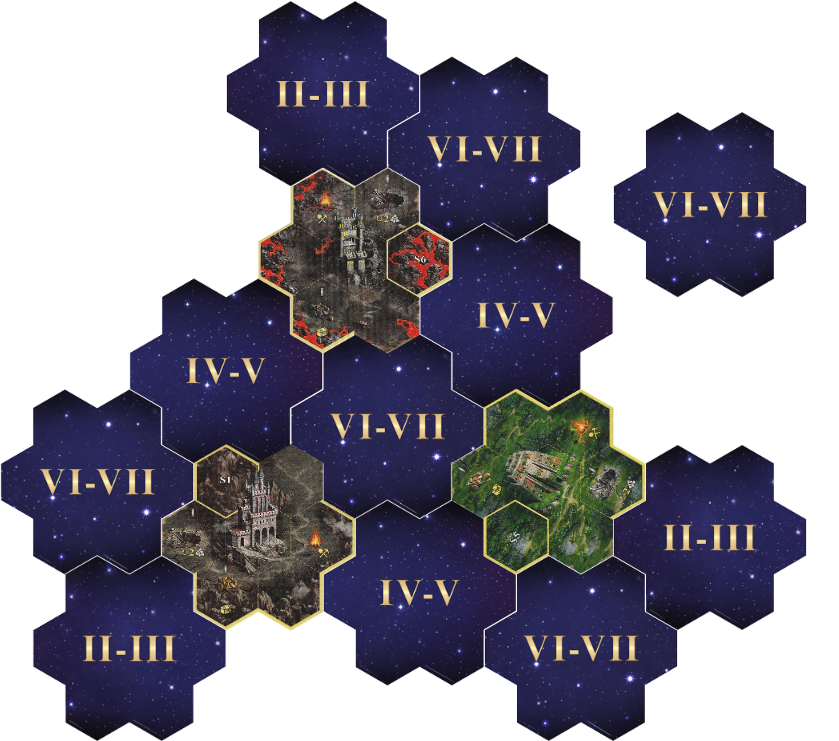
\includegraphics[width=0.56\linewidth]{\maps/king_of_the_hill_v2-3p.png}};

  \blocked{13.71}{-2.62}{90}
  \blocked{11.28}{-5.39}{90}
  \blocked{14.91}{-6.09}{90}

  \node at (17.5, -0.5) {\large{{\textbf{\textcolor{darkcandyapplered}{C1/C3}}}}};

  \node at (13.33, -4.53) {{{\footnotesize{The}}}};
  \node at (13.33, -4.82) {{{\footnotesize{Hill}}}};

  \node at (13.4, -9.5) {\textbf{3-PLAYER SCENARIO}};

  \node at (4.6, -1.8) {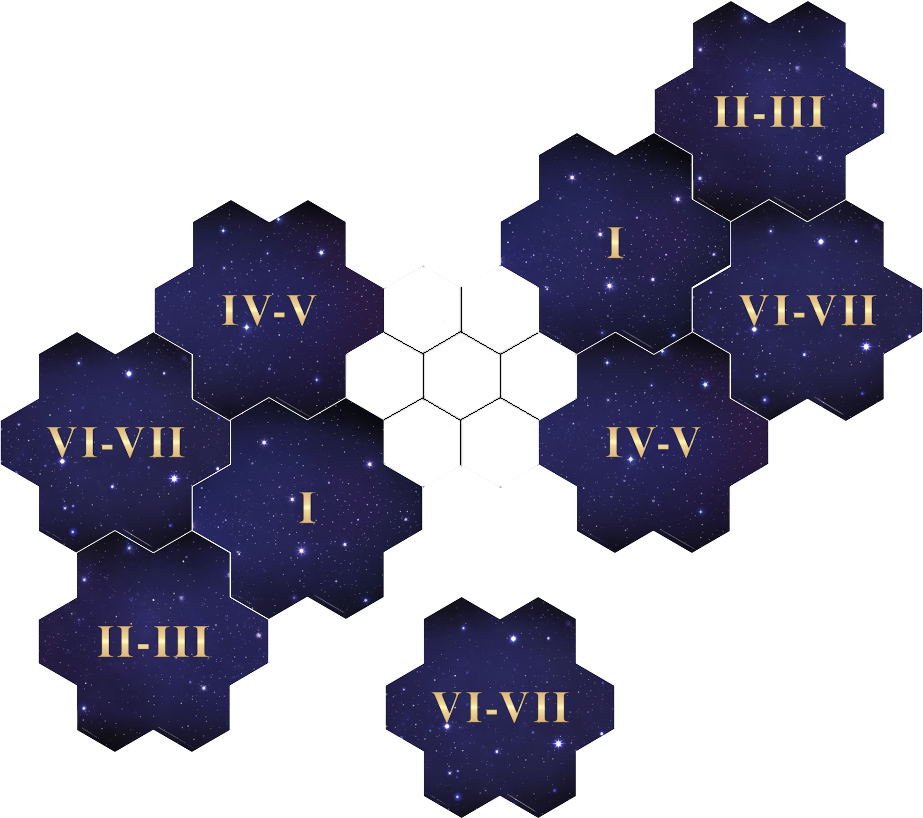
\includegraphics[width=0.54\linewidth]{\maps/king_of_the_hill_v2-2p.png}};

  \blocked{6.63}{-0.76}{90}
  \blocked{2.57}{-2.15}{90}

  \node at (6.8, -4.4) {\large{{\textbf{\textcolor{darkcandyapplered}{C1/C3}}}}};

  \node at (4.61, -1.29) {{{\footnotesize{The}}}};
  \node at (4.61, -1.58) {{{\footnotesize{Hill}}}};

  \node at (4.6, -7.0) {\textbf{2-PLAYER SCENARIO}};
\end{tikzpicture}

